Nun bekannte wichtige Formeln:
\begin{equation*}
\underset{\to M}{\underbrace{\underset{\Rightarrow R}{\underbrace{\sigma T_\text{eff}^4=\frac{L}{4\pi R^2} \qquad \underset{\Rightarrow L}{\underbrace{S=\frac{L}{4\pi D^2}}}}} \qquad g=\frac{GM}{R^2}}}
\end{equation*}
\begin{equation*}
\frac{L}{L_\odot}\approx\left(\frac{M}{M_\odot}\right)^\frac{7}{2}
\end{equation*}
\subsection{Enternungsbestimmungen}
\subsubsection{Trigonometrische Parallaxe}
\begin{itemize}
\item rein geometrische Methode
\begin{figure}[H]
\begin{multicols}{2}
\begin{figure}[H]
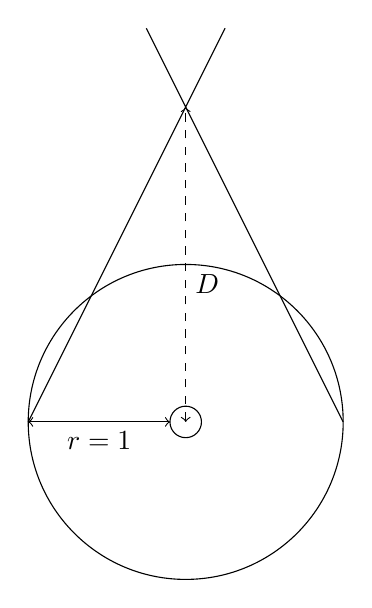
\begin{tikzpicture}
\draw (0,0)circle(2 cm)circle(0.2 cm);
\draw[<->] (-2,0)--(-0.2,0)node[midway,below]{$r=\SI{1}{\au}$};
\draw (-2,0)--(0.5,5)(-0.5,5)--(2,0);
\draw[<->,dashed] (0,0)--(0,4)node[midway,below right]{$D$};
\end{tikzpicture}
\end{figure}\columnbreak
\begin{align*}
\SI{1}{\au}&=\SI{1.496e13}{\cm}\\
\text{(astro}&\text{nomische Einheit)}\\
\text{große}&\text{ Halbachse der Erde}\\
\frac{r}{D}&=\tan(\varphi)\approx\varphi
\end{align*}
\end{multicols}
\end{figure}
\item \underline{Def}: $\SI{1}{\pc}$ ist der Abstand $D$, der bei einem Winkelunterschied von 1 Bogensekunde vorliegt.
\item Es gilt: $D=\left(\frac{\varphi}{1\text{"'}}\right)^{-1}\si{\pc}$
\begin{itemize}
\item Bessel 1837: Abstand zu "`G1Cygni"'
\item Erdbewegung der Teleskope: $\Delta p\sim \SI{0.01}{\gr} \to D\leq \SI{30}{\pc}$\\
Satellit HIPPARCOS: $\Delta p\sim \SI{0.001}{\gr} \to D\leq \SI{300}{\pc}$\\
aktuell: GAIA: $\Delta p \sim \SI{2e-4}{\gr}$
\end{itemize}
\end{itemize}
\subsubsection{Eigenbewegungen}
\begin{itemize}
	\item Sterne bewegen sich relativ zur Sonne!
		\begin{itemize}[label={$\cdot$}]
			\item radiale Komponente der Geschwindigkeit (mit Hilfe von Spektrallinien bestimmbar):
				\begin{equation*}
					v_r=\frac{\Delta \lambda}{\lambda_0}\cdot c=\frac{\lambda-\lambda_0}{\lambda_0}\cdot c
				\end{equation*}
				$\lambda$: gemessene Wellenlänge $\neq\lambda_0$ aufgrund der Dopplerverschiebung\\
				$\lambda_0$: Ruhewellenlänge des atomaren Übergangs (messbar im Labor)
		\end{itemize}
	\item[] Koncetion:
		\begin{itemize}
			\item[] $v_r>\sigma$ Bewegung von uns weg (Rotverschiebung)
			\item[] $v_r<\sigma$ Bewegung zu uns hin
		\end{itemize}
	\item tangentiale Komponente:\\
		messbar über die Eigenbewegung $\mu$ des Sterns auf der Himmelssphäre (in $\si{\gr\per\year}$)
		\begin{equation*}
			v_t=D\cdot \mu \Leftrightarrow \frac{v_t}{\si{\km\per\s}}=\num{4.74}\left(\frac{D}{\SI{1 }{\pc}}\right)\cdot\left(\frac{\mu}{\SI{1}{\gr\per\year}}\right)=\left(\frac{\si{\pc}}{\si{\gr}}\right)
		\end{equation*}
		HIPPARCOS:
		$\mu$ für ca $10^5$ Sterne
		\begin{itemize}
			\item $v_t$ sowie $D$ bekannt
			\item Datenbank mit Sterngeschwindigkeiten
			\item Struktur der Galaxis
		\end{itemize}
\end{itemize}
\subsubsection{Sternstromparallaxe}
\begin{itemize}
	\item Sterne eines offenen Sternhaufens haben alle eine sehr ähnliche Raumgeschwindigkeit $\vec{v}$
	\item Die Position des $i$-ten Sterns wird beschrieben durch:
		\begin{equation*}
			\vec{r_i}(t)=\vec{r_i}(0)+\vec{v}\cdot t
		\end{equation*}
		\begin{itemize}
			\item Richtungsvektor: $\vec{n_i}(t)=\frac{\vec{r_i}(t)}{\left|\vec{r_i}(t)\right|} \underset{t\to\infty}{\to} \frac{\vec{v}{\left|\vec{v}\right|}}=\hat{n}_\text{conv}$
		\end{itemize}
		\begin{figure}[H]
			\begin{tikzpicture}
				\node[name=u] at (0,0){};
				\node[name=s1] at (-0.5,4){};
				\node[name=s2] at (-0.5,5){};
				\node[name=k,right] at (2,4.5){$K$};
				\draw[dashed] (u)node[left]{$\vec{r_i}$}--(s2)node[midway,left]{$\hat{n_i}$}(s2)node[above]{$\vec{v_t}$}--(k)(s1)node[below]{$\vec{v_t}$}--(k)(u)--(k)node[midway,right]{$\hat{n}_\text{conv}$};
			\end{tikzpicture}
		\end{figure}
		$\Psi$ ist die Sternstromparallaxe, gegeb durch den Winkel zwischen $\hat{n}$ und $\hat{n}_\text{conv}$
	\item Es gilt: $\cos(\Psi)=\hat{n}\cdot\hat{n}_\text{conv}=\hat{n}\cdot\frac{\vec{v}}{|\vec{v}|}$
		\begin{itemize}
			\item $v_r=v\cos(\Psi),\ v_t=\sin(\Psi)$
			\item $v_t=v_r\cdot\tan(\Psi)$
		\end{itemize}
	\item Weiterhin gilt: $v_t=D\cdot\mu$
		\begin{itemize}
			\item $D=\frac{v_r\tan(\Psi)}{\mu}\ \Rightarrow$ Messung von $v_r$ und $\Psi$ und $\mu$ zwischen Beobachter und Sternhaufen
		\end{itemize}
	\item \underline{Beispiele}:
		\begin{itemize}[label={}]
			\item Hyaden: $D\approx \SI{45}{\pc}$
			\item Ursa-Major $D\approx \SI{24}{\pc}$
			\item Plejaden $D\approx \SI{130}{\pc}$
		\end{itemize}
	\item historisch bedeutsam, da Methode für Enternungen $>\SI{30}{\pc}$ (unterste Sprosse der Enternunsgleiter)
\end{itemize}
\subsubsection{Photometrische Entfernung}
\begin{itemize}
	\item \underline{Idee}: Sterne auf der Hauptreihe habe für eine gegebene Farbe die gleiche Leuchtkraft
	\item Für einen Sternhaufen (allen Sterne haben $\approx $ gleiche Entfernung $D$ von uns) kann man ein Farben-Helligkeitsdiagramm mit Hauptreihe erhalten, bei dem die scheinbare Helligkeit aufgetragen ist
	\item In einem zweiten Schritt erhält man das Entfernungsmodul ($m-M$), indem man die Haupreihe mit einer geeichten Hauptreihe (Sternhaufen in der Nähe, z. B. Hyaden) in Übereinstimmung bringt
		\begin{equation*}
			m-M=5\log\left(\frac{D}{\si{\pc}}\right)-5
		\end{equation*}
		\begin{figure}[H]
			\centering
			\begin{tikzpicture}
				\draw[->] (-1,0)--(5,0)node[below right]{$B-V=m_B-m_V$};
				\draw[->] (0,-1)--(0,5)node[above left]{$M$};
				\foreach \x \y in {-5/5,0/4,5/3,10/2,15/1}{
					\draw (0.1,\y )--(-0.1,\y )node[left]{\x };
				};
				\draw (0.5,4.5)--(4.5,0.5);
			\end{tikzpicture}
		\end{figure}
	\item \underline{Probleme}:
		\begin{itemize}[label={$\cdot$}]
			\item Stern wandert auf Hauptreihe während er altert
			\item HR-Sterne sind Zwerge der Klasse V (schwache Leuchtkraft)
			\item Extinktion\\
				Extinktion: Die Beziehung zwischen absoluter und scheinbarer Helligkeit wird durch die Absorption und Streuung des Sternenlichtes geändert.
		\end{itemize}
	\item Strahlungstransportgleichung ($\to$ 2.2) ohne Emission:
		\begin{align*}
			\frac{dI_\nu}{ds}&=-\kappa_\nu I_\nu\\
			\Rightarrow I_\nu(s)&=I_\nu(0)\cdot e^{-\tau_\nu(s)} \text{ mit } \tau_\nu(s)=\int\limits_{0}^sds'\kappa_\nu(s') \text{ optische Tiefe}
		\end{align*}
	\item $s_\nu=s_\nu(0)e^{-\tau_\nu(s)}$
	\item[$\mathbf{\to}$] Extinktionskoeffizient:
		\begin{equation*}
			A_\nu := m-m_0=-\num{2.5}\log\left(\frac{S_\nu}{S_\nu(0)}\right)=\num{2.5}\log(e)\tau_\nu=\num{1.086}\tau_\nu
		\end{equation*}
		mit: $m$ Magnitude mit Absorption und $m_0$ Magnitude ohne Absorption
		\begin{itemize}
			\item Quelle erscheint schwächer und ihre Farbe ändert sich, da Extinktion von $\nu$ abhängt (via $\kappa_\nu$) $\to$ Sterne erscheinen röter als sie sind
		\end{itemize}
	\item Beschreibung mit Hilfe des Farbexzesses (für Filter $X$ und $Y$)
		\begin{equation*}
			E(X-Y):=A_X-A_Y=(X-X_0)-(Y-Y_0)=(X-Y)-(X-Y)_0
		\end{equation*}
	\item Verhältnis $\frac{A_X}{A_Y}=\frac{\tau_{\nu ,X}}{\tau_{\nu, Y}}$ hängt nur von optischen Eigenschaften des Staubes ab.
		\begin{itemize}
			\item $E(X-Y)=A_X-A_Y=A_Y\left(\frac{A_X}{A_Y}-1\right)=A_Y\cdot\frac{1}{R_Y}$\\
				üblicherweise: $X=B$ und $Y=V$
			\item $A_V=R_VE(B-V)$\\
				z.B. Staub der Milchstraße (empirisch):
				\begin{equation*}
					A_V=(\num{3.1}\pm\num{0.1})E(B-V)
				\end{equation*}
				In der Sonnenumgebung (nnerhalb der Scheibe)
				\begin{equation*}
					A_V \sim \SI{1}{\mag}\frac{D}{\SI{1}{k\pc}}
				\end{equation*}
			\item nicht vernachlässigbar bei der photometrischen Entfernungsbestimmung von Sternhaufen
			\item Prozedur in 2 Schritten:
				\begin{enumerate}[label={$(\roman*)$}]
					\item Erstelle Zweifarben-Diagramm des Sternhaufens
						\begin{figure}[H]
							\begin{tikzpicture}
							\end{tikzpicture}
						\end{figure}
						\begin{itemize}[label={$\to$}]
							\item Verschiebung der HR des Sternhaufens entlang des Verfärbungsvektors bis zur Übereinstimmung der geeichten HR (ohne Absorption)
								\begin{itemize}[label={$\Rightarrow$}]
									\item $E(B-V)\Rightarrow A_V=\num{3.1}E(B-V)$
								\end{itemize}
						\end{itemize}
					\item Bestimmung des Entfernungsmoduls durch vertikale Verschiebung der Hauptreihe um Farben-Helligkeits-Diagramm bis zur Übereinstimmung mit einer geeichten HR.
						\begin{equation*}
							m-M=5\log\left(\frac{D}{\SI{1}{\pc}}\right)-5+\underset{\underset{(m-m_0)}{\uparrow}}{A_V}
						\end{equation*}
				\end{enumerate}
		\end{itemize}
\end{itemize}
\subsubsection{Visuelle Doppelsterne}
\begin{figure}[H]
	\begin{multicols}{2}
		\begin{figure}[H]
			\centering
			\begin{tikzpicture}
				\node at (0,0.8){$\Theta$};
				\coordinate (B) at (0,0);
				\coordinate (A) at (-0.5,1);
				\coordinate (C) at (0.5,1);
				\draw (B)--(A);
				\draw (B)--(C);
				\pic[draw,angle eccentricity=3] {angle=C--B--A};
			\end{tikzpicture}
		\end{figure}\columnbreak
		mit Massen $m_1$ und $m_2$\\
		Keplersches Gesetz: $P^2=\frac{4\pi^2a^3}{G(m_1+m_2)}$
	\end{multicols}
\end{figure}
\begin{itemize}
	\item Messung von Periode $P$ und Winkeldurchmesser der Bahn $2\Theta$ \& Bestimmung von $m_1$ und $m_2$ mit Hilfe ihrer spektralen Eigenschaften $\Rightarrow a \Rightarrow $ Abstand $D=\frac{a}{\Theta}$
\end{itemize}
\subsubsection{Entfernung pulsierender Sterne}
\begin{itemize}
	\item Verschiedene Arten pulsierender Sterne zeigen periodische Helligkeitsänderungen, wobei ihre Periode mit der Masse (und daher der Leuchtkraft) der Sterne korrelliert ist.
	\item Man findet (s. Übung)
		\begin{equation*}
			P  \sim \bar{\rho}^{-\frac{1}{2}}
		\end{equation*}
		wobei $\bar{\rho}\sim\frac{M}{R^3}$ mittlere Dichte des Sterns
	\item weiterhin gilt: $L\sim M^3$ und $L\sim R^3\cdot T_{eff}$
		\begin{itemize}
			\item $P\sim\frac{R^\frac{3}{2}}{\sqrt{M}}\sim L^\frac{7}{12}$, falls $T_{eff}=const$
		\end{itemize}
	\item[$\Rightarrow$] drei Sorten pulsierender Sterne:
		\begin{enumerate}[label={$(\roman*)$}]
			\item $\delta$-Cephei (klass. Cepheiden): junge Sterne
				\begin{equation*}
					\mathcal{M}_\nu =-3\log\left(\frac{P}{\SI{1}{\d}}\right)-\num{0.8} \ \text{(aus Experimenten)}
				\end{equation*}
				Zur Minimierung der Extinktion und Streuung Beobachtung der $P-L$-Relation in Nah-IR besonders nützlich.
			\item W Virginis Sterne (Population II, Cepheiden):\\
				massearme, $\underset{\text{schwerer als Helium}}{\text{metallarme}}$ Sterne
			\item RR Lyrae-Sterne (ebenfalls Population II)\\
				Metallarm\\
				sehr langsame Perioden $\mathcal{M}_\nu \in [\num{0.5};\num{1.0}]$ mit $\mathcal{M}_F=(-\num{2.0}\pm\num{0.3})\log\left(\frac{P}{\SI{1}{\d}}\right)+\num{0.06}\cdot\left[\frac{\text{Fe}}{\text{H}}\right]-\num{0.7}$
		\end{enumerate}
		I.a. für ein Element X: $\left[\frac{\text{X}}{\text{H}}\right]=\log\left(\frac{n(\text{X})}{n(\text{H})}\right)_\ast-\log\left(\frac{n(\text{X})}{n(\text{H})}\right)_\odot$ wobei $n(\text{X})$= Anzahl der Spezies X\\
		z.B. $\left[\frac{\text{Fe}}{\text{H}}\right]=-\num{1}\Rightarrow$ Eisen im Stern hat ein zehntel der solaren Häufigkeit\\
		Metallizität $Z$: Massenzahl aller Elemente schwerer als Helium\\
		z.B.: $Z_\odot=\num{0.02}\Rightarrow \SI{98}{\%}$ der Sonnenbasse besteht aus H und He
\end{itemize}
\underline{Endergebnis}: typische astronomische Distanzen:
\begin{itemize}[label={}]
	\item Sonne $\SI{1}{\au}\approx \SI{150e6}{\km}$ ($\SI{8}{\min}\ \SI{15}{\s}$ für ein Photon)
	\item $\alpha$Centauri $\SI{1.3}{\pc}$
	\item Dicke der Galaxie $\SI{0.3}{k\pc}$
	\item Abstand zum galaktischen Zentrum $\SI{8}{k\pc}$
	\item Radius der Galaxis $\SI{12.5}{k\pc}$
	\item nächste Galaxie $\SI{55}{k\pc}$
	\item Andromeda M31 $\SI{770}{k\pc}$
	\item Größe eines Galaxiehaufens $\num{1}-\SI{5}{M\pc}$
	\item Zentrum des nächsten Superhaufens (Virgo) $\SI{20}{M\pc}$
	\item Größe eines Superhaufens $\SI{260}{M\pc}$
	\item sichtbares Universum $\SI{4000}{M\pc}$
\end{itemize}
